
% Setup
    \documentclass[a4paper, 10pt, conference]{ieeeconf}
    \IEEEoverridecommandlockouts                              % This command is only
                                                              % needed if you want to
                                                              % use the \thanks command
    \overrideIEEEmargins
    % See the \addtolength command later in the file to balance the column lengths
    % on the last page of the document

    \usepackage[utf8]{inputenc}
    \usepackage[T1]{fontenc}
    \usepackage{xcolor}
    \usepackage[
bibstyle=ieee,
isbn = false,
doi = false,
url = false,
eprint=false]{biblatex}


\AtEveryBibitem{\clearfield{address}}
\AtEveryBibitem{\clearlist{language}}

\addbibresource{refs.bib}

\DefineBibliographyStrings{english}{
  phdthesis   = Ph\adddot D\adddot\addspace thesis,
  mathesis    = Master's thesis,
}

% https://ftp.snt.utwente.nl/pub/software/tex/macros/latex/contrib/biblatex-contrib/biblatex-ieee/ieee.bbx

%swapped chapter+pages with published+location date:

\DeclareBibliographyDriver{inproceedings}{%
  \usebibmacro{bibindex}%
  \usebibmacro{begentry}%
  \usebibmacro{author/translator+others}%
  \setunit{\labelnamepunct}\newblock
  \usebibmacro{title}%
  \newunit
  \printlist{language}%
  \newunit\newblock
  \usebibmacro{byauthor}%
  \newunit\newblock
  \usebibmacro{maintitle+booktitle(inproceedings)}%
  \midsentence
  \newunit\newblock
  \usebibmacro{event+venue+date}%
  \newunit\newblock
  \usebibmacro{byeditor+others}%
  \newunit\newblock
  \printfield{volumes}%
  \newunit\newblock
  \usebibmacro{series+number}%
  \newunit\newblock
  \printfield{note}%
  \newunit\newblock
  \printlist{organization}%
  \newunit\newblock
  \usebibmacro{volume+part}%
  \newunit\newblock
  \usebibmacro{chapter+pages}% %swapped chapter+pages with published+location date
  \newunit
  \usebibmacro{publisher+location+date}%
  \newunit\newblock
  \iftoggle{bbx:isbn}
    {\printfield{isbn}}
    {}%
  \newunit\newblock
  \usebibmacro{doi+eprint+url}%
  \newunit\newblock
  \usebibmacro{addendum+pubstate}%
  \setunit{\bibpagerefpunct}\newblock
  \usebibmacro{pageref}%
  \newunit\newblock
  \iftoggle{bbx:related}
    {\usebibmacro{related:init}%
     \usebibmacro{related}}
    {}%
  \usebibmacro{finentry}}
  
  
  %swapped chapter+pages with published+location date:
  
  \DeclareBibliographyDriver{incollection}{%
  \usebibmacro{bibindex}%
  \usebibmacro{begentry}%
  \usebibmacro{author/translator+others}%
  \setunit{\labelnamepunct}\newblock
  \usebibmacro{title}%
  \newunit
  \printlist{language}%
  \newunit\newblock
  \usebibmacro{byauthor}%
  \newunit\newblock
  \usebibmacro{in:}%
  \usebibmacro{maintitle+booktitle}%
  \newunit\newblock
  \usebibmacro{series+number}%
  \newunit\newblock
  \usebibmacro{byeditor+others}%
  \newunit\newblock
  \printfield{edition}%
  \newunit
  \iffieldundef{maintitle}
    {\printfield{volume}%
     \printfield{part}}
    {}%
  \newunit
  \printfield{volumes}%
  \newunit\newblock
  \printfield{note}%
  \newunit\newblock
  \usebibmacro{chapter+pages}%
  \newunit\newblock
  \usebibmacro{publisher+location+date}%
  \newunit\newblock
  \iftoggle{bbx:isbn}
    {\printfield{isbn}}
    {}%
  \newunit\newblock
  \usebibmacro{doi+eprint+url}%
  \newunit\newblock
  \usebibmacro{addendum+pubstate}%
  \setunit{\bibpagerefpunct}\newblock
  \usebibmacro{pageref}%
  \newunit\newblock
  \iftoggle{bbx:related}
    {\usebibmacro{related:init}%
     \usebibmacro{related}}
    {}%
  \usebibmacro{finentry}}


    % The following packages can be found on http:\\www.ctan.org
    \usepackage{graphics} % for pdf, bitmapped graphics files
    \usepackage{epsfig} % for postscript graphics files
    \usepackage{mathptmx} % assumes new font selection scheme installed
    \usepackage{mathptmx} % assumes new font selection scheme installed
    \usepackage{amsmath} % assumes amsmath package installed
    \usepackage{amssymb}  % assumes amsmath package installed

    \title{\LARGE \bf
    Experimental Validation of Reference Spreading for Robotic Manipulation of Unmodeled Objects
    }

    %\author{ \parbox{3 in}{\centering Huibert Kwakernaak*
    %         \thanks{*Use the $\backslash$thanks command to put information here}\\
    %         Faculty of Electrical Engineering, Mathematics and Computer Science\\
    %         University of Twente\\
    %         7500 AE Enschede, The Netherlands\\
    %         {\tt\small h.kwakernaak@autsubmit.com}}
    %         \hspace*{ 0.5 in}
    %         \parbox{3 in}{ \centering Pradeep Misra**
    %         \thanks{**The footnote marks may be inserted manually}\\
    %        Department of Electrical Engineering \\
    %         Wright State University\\
    %         Dayton, OH 45435, USA\\
    %         {\tt\small pmisra@cs.wright.edu}}
    %}

    \author{Gijs van den Brandt% <-this % stops a space
    % \thanks{*This work was made in accordance with the TU/e Code of Scientific Conduct for the Master thesis}% <-this % stops a space
    % \thanks{$^{1}$H. Kwakernaak is with Faculty of Electrical Engineering, Mathematics and Computer Science,
    %         University of Twente, 7500 AE Enschede, The Netherlands
    %         {\tt\small h.kwakernaak at papercept.net}}%
    % \thanks{$^{2}$P. Misra is with the Department of Electrical Engineering, Wright State University,
    %         Dayton, OH 45435, USA
    %         {\tt\small p.misra at ieee.org}}%
    }

  \usepackage{pdfpages}

    \begin{document}


  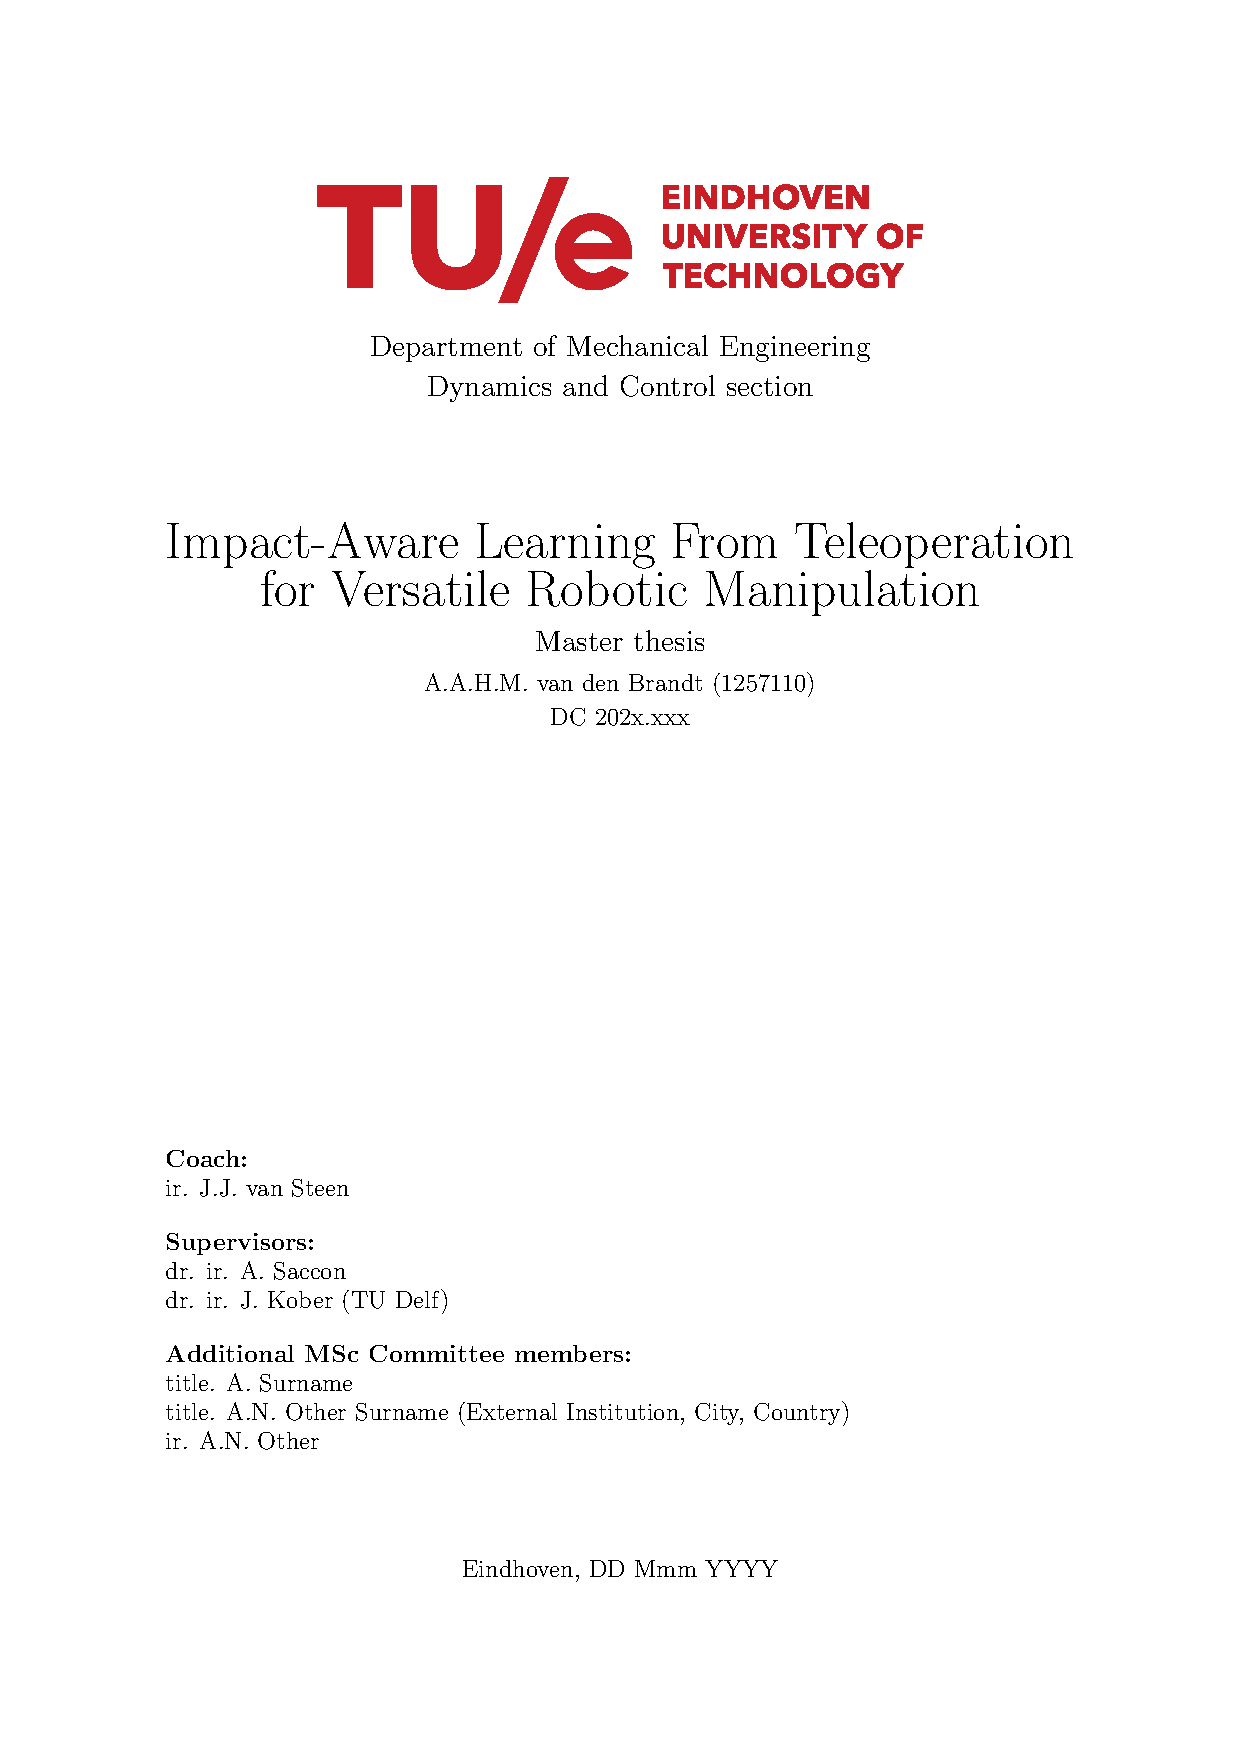
\includepdf{Thesis.pdf}
    \maketitle
    \thispagestyle{empty}
    \pagestyle{empty}

% Abstract
    \begin{abstract}

    This electronic document is a ``live'' template. The various components of your paper [title, text, heads, etc.] are already defined on the style sheet, as illustrated by the portions given in this document.

    \end{abstract}

% Introduction
    \section{INTRODUCTION}

    Automation has historically played a crucial role in the logistics industry. Our current way of living depends on autonomous systems for global transportation and warehousing. The growing labor shortage and increasing demand for online retail motivate further developments in the logistics sector~\cite{dekhneAutomationLogisticsBig2019}.

    An example of automation in logistics can be found in depalletizing, where object are removed from a pallet. Three different depalletizing approaches can be found in industry. 

    A logistical aspect where machines struggle to fully compete with humans is object manipulation. A practical examples of this is depalletizing. While robots are strong and consistent when manipulating objects, humans are versatile and swift. Robots are held back from faster performance because they must often slow down prior to making contact; establishing contact at a high velocity -- an event referred to as an impact -- could cause damage to the robot or its environment. On the contrary, humans intrinsically exploit impacts in the form of grabbing, bouncing and hitting. \textcolor{red}{(give better explanation of depalletizing: manual and automatic approach)}

    The field of impact-aware control aims to better equip robots for making contact at high velocities. These impacts are paired with large contact forces that could damage the system. Previous work describes control using the maximum allowable impact velocity that complies with safety constraints such as limits for the contact force~\cite{dehioRobotSafeImpactsSoft2021, dehioDualArmBoxGrabbing2022}. This was combined with a compliant cover for the robot that reduces contact forces at impact, facilitating higher feasible impact velocities. Rather than using a soft cover, compliancy may also be achieved by designing a robot with low inertia and high backdrivability as was done in \cite{songDevelopmentLowInertiaHighStiffness2018}.

    In addition to the large contact forces, a subject of interest is the velocity jump at the time of impact. Time misalignments between velocity jumps in the reference and in the actual system cause the velocity tracking error to peak\cite{biemondTrackingControlMechanical2012}, as is shown in Figure xxx. This error peak results in undesired control effort and should therefore be avoided. In \cite{yangImpactInvariantControl2021}, the robot's velocities are projected into an impact-invariant subspace based on the expected point of impact. As a result, impact-driven peaks in the velocity tracking error are reduced significantly. It is not always possible to describe a point of impact, however. Often times, impacts occur between surfaces rather than just points. Furthermore, corners of the surface may impact at diverging intervals in uncertain order during what is called near-simultaneous impacts, shown in Figure xxx.

    The impact-aware control scheme called Reference Spreading \cite{sacconSensitivityAnalysisHybrid2014} addresses error peaking caused by misaligned impacts. It operates on the basis of a tracking error that switches once an impact is detected. This concept is best explained at the hand of Figure xxx. The reference is split at the nominal impact time into an ante- and post impact reference. These references are then extended. Initially, the tracking error is based on the extended ante-impact reference, but this is switched to the post-impact reference once an impact is detected. Evidently, this can reduce the error peaking.

    Reference spreading can also handle simultaneous impacts. \cite{vansteenRobotControlSimultaneous2021} \textcolor{red}{(explanation)}

    By addressing the peaking error, reference spreading facilitates faster object manipulation, making it interesting to industry if its effectivity can be proven in practice. Reference spreading for object manipulation has already been validated in simulations \cite{vansteenRobotControlSimultaneous2021,zwartImpactAwareLearningDemonstration2019}. Experimental validations have been limited to interaction with a fixed environment, however \cite{rijnenReferenceSpreadingTracking2020,uitendaalTeachingRobotsInteraction2022}. The goal of this work is therefore to \textbf{provide a real-world implementation of reference spreading for practical object manipulation tasks.} To translate the results from simulation to reality, the following contributions are made:

    \textbf{1. Motion planning for impacts without object models}: Generating a reference with velocity jumps that is coherent with the system’s dynamics is challenging. 
    One approach maps the ante-impact velocity to the post-impact velocity based on conservation of momentum [ref for impact map]. This requires a model of the environment, which is feasible in simulations with simplified dynamics, but challenging in reality.
    Impact-driven velocity jumps could instead be inferred experimentally. In previous studies \cite{aouajPredictingPostImpactVelocity2021}, the control gains are reduced to zero upon detection of the impact while inferring an impact map, so that the velocity jump would not result in excessive motor torques.
    A different model-free motion planning strategy is proposed, which not only produces velocity-reference jumps that are coherent with the system dynamics, but also leverages human intuition to generate fluid motions before and after the impact. This is achieved by introducing a human in the loop by means of teleoperation. %(This strategy introduces a human in the loop by means of teleoperation; the operator performs a demonstration, after which a reference can be extracted. During the demonstration, the control gains are relatively low. This mitigates the torque jumps at the time of impact, meaning that the controller does not need to be turned off. The teleoperator instinctively accounts for the low control gains and can perform precise motion tasks despite poor tracking of the controller.)

    \textbf{2. Impact detection}: The reference spreading scheme should switch between ante-, intermediate-, and post-impact references at the appropriate time. This requires an impact detection algorithm. Approaches in literature look either at position data \cite{rijnenMotionSignalsVelocity2018} or external force estimations \cite{uitendaalTeachingRobotsInteraction2022,properAimAwareCollisionMonitoring2021,properValidationNumericalSimultaneous2022} for signs that could be caused by impacts. We show that these signs are necessary, but not sufficient conditions for an impact -- only looking at position or contact force can result in false positives. To limit false detection of impacts, a novel impact detector that looks at both force and position data is proposed and evaluated.

    \textbf{3. Custom end effector:}

    \textbf{\textcolor{red}{(4. Intermediate impact phase controller:)}}

% Background
    \section{Background}
    \subsection{Compliant robots}
    \subsection{Quadratic programing control}
    \subsection{Reference spreading}
    \subsection{Impact detection}
    \section{Tracjectory planning}

% Methods
    \section{Methods}
    \subsection{Soft end effector}
    \subsection{Trajectory planning via teleoperation}
    \subsection{Reference spreading formulation}

% Experimental validation
    \section{Experimental validation}
    \subsection{Implementation}
    \subsection{End effector evaluation}
    \subsection{Reference spreading}
    \subsection{Intermediate modes}

% Conclusion
    \section{Conclusion}
    
% Appendix
\clearpage
\section*{appendix}
\subsection{Rotation mathematics}
\subsection{End effector design}
\subsection{Supplementary experimental results}
hoi

\end{document}

